Predicting the future trajectory of multiple agents is a critical task with applications in autonomous driving \cite{argoverse}, social behavioral modeling \cite{sun2021multi}. %, and hurricane tracking \cite{hall2007statistical}
In practice, the problem is difficult due to the inherent stochasticity of human motion, and the strong inter-dependency among the agents where the number of interactions grows quadratically with the number of agents. Moreover, agent movements are often influenced by environmental features such as road markings, boundaries, and social preference, which are impossible to measure and model effectively. Such a partially observed setting introduces a significant amount of uncertainty. 
%. In practice, it is impossible to exactly measure all dependencies among the agents and the influence of the environment. 

Many recent works on learning multi-agent dynamics has shifted to probabilistic modeling as a principled framework to represent uncertainty \cite{mfp, trajectron++}. However, common metrics used in probabilistic trajectory predictions works, such as minimum average displacement of 6 samples (minADE) , do not fully reflect the quality of probabilistic forecasts. A probabilistic prediction should be \textit{calibrated} and \textit{sharp}; that is, the predicted distribution must cover likely future scenarios without being so broad and uncertain as to be useless. 

\begin{figure}[t]
    \centering
    \begin{subfigure}[b]{0.35\textwidth}
        \centering
        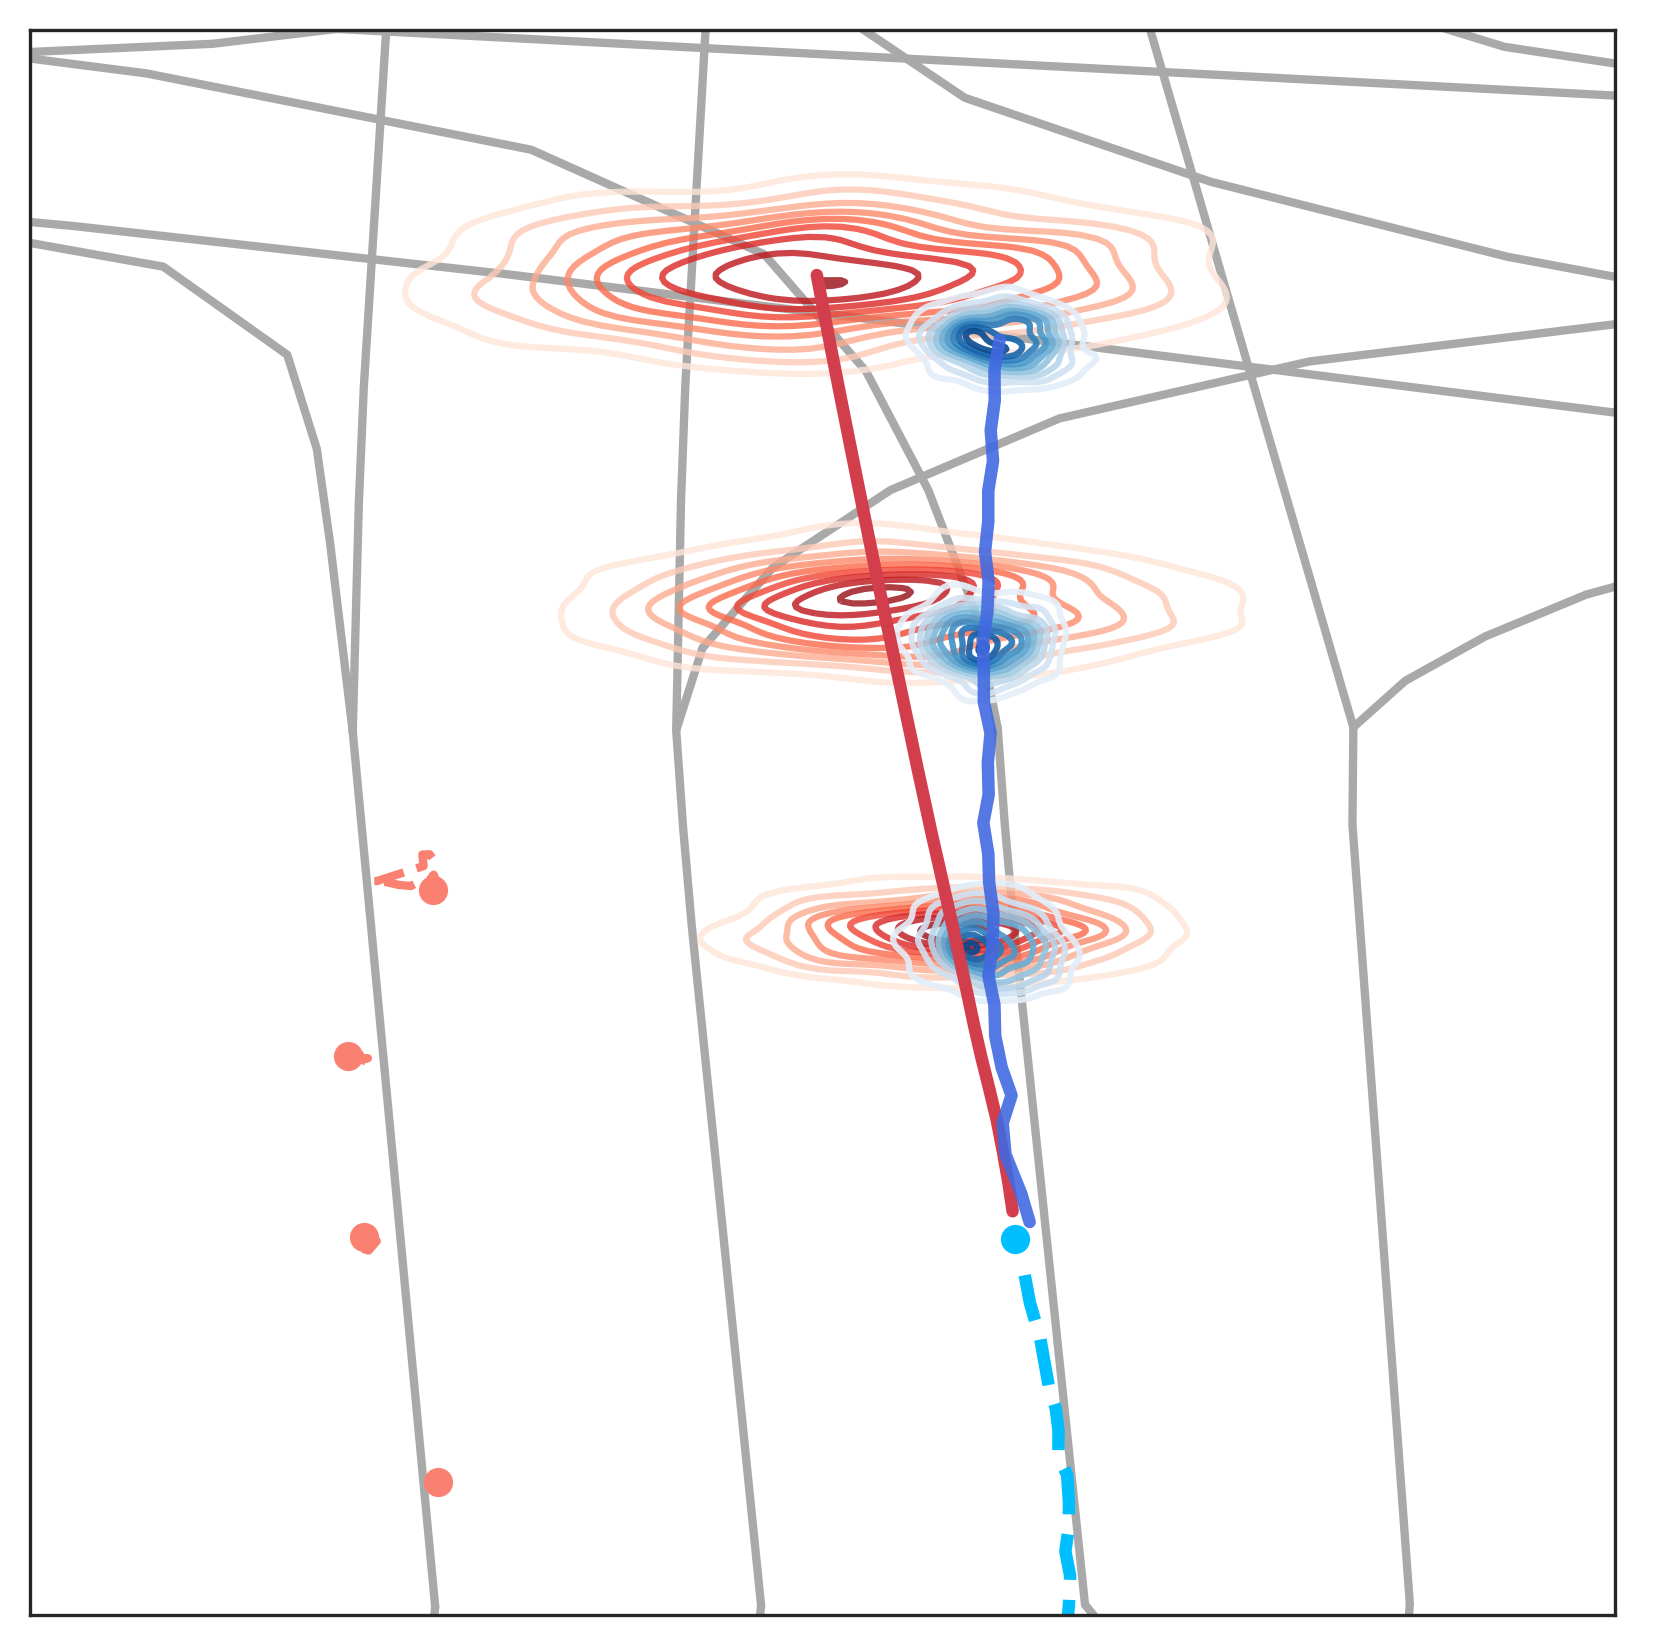
\includegraphics[width=\textwidth]{equivariance/figs/rot1.png}
        \caption{Original scene}
        \label{fig:noneq0}
    \end{subfigure}
    \hspace{2em}
    \begin{subfigure}[b]{0.35\textwidth}
        \centering
        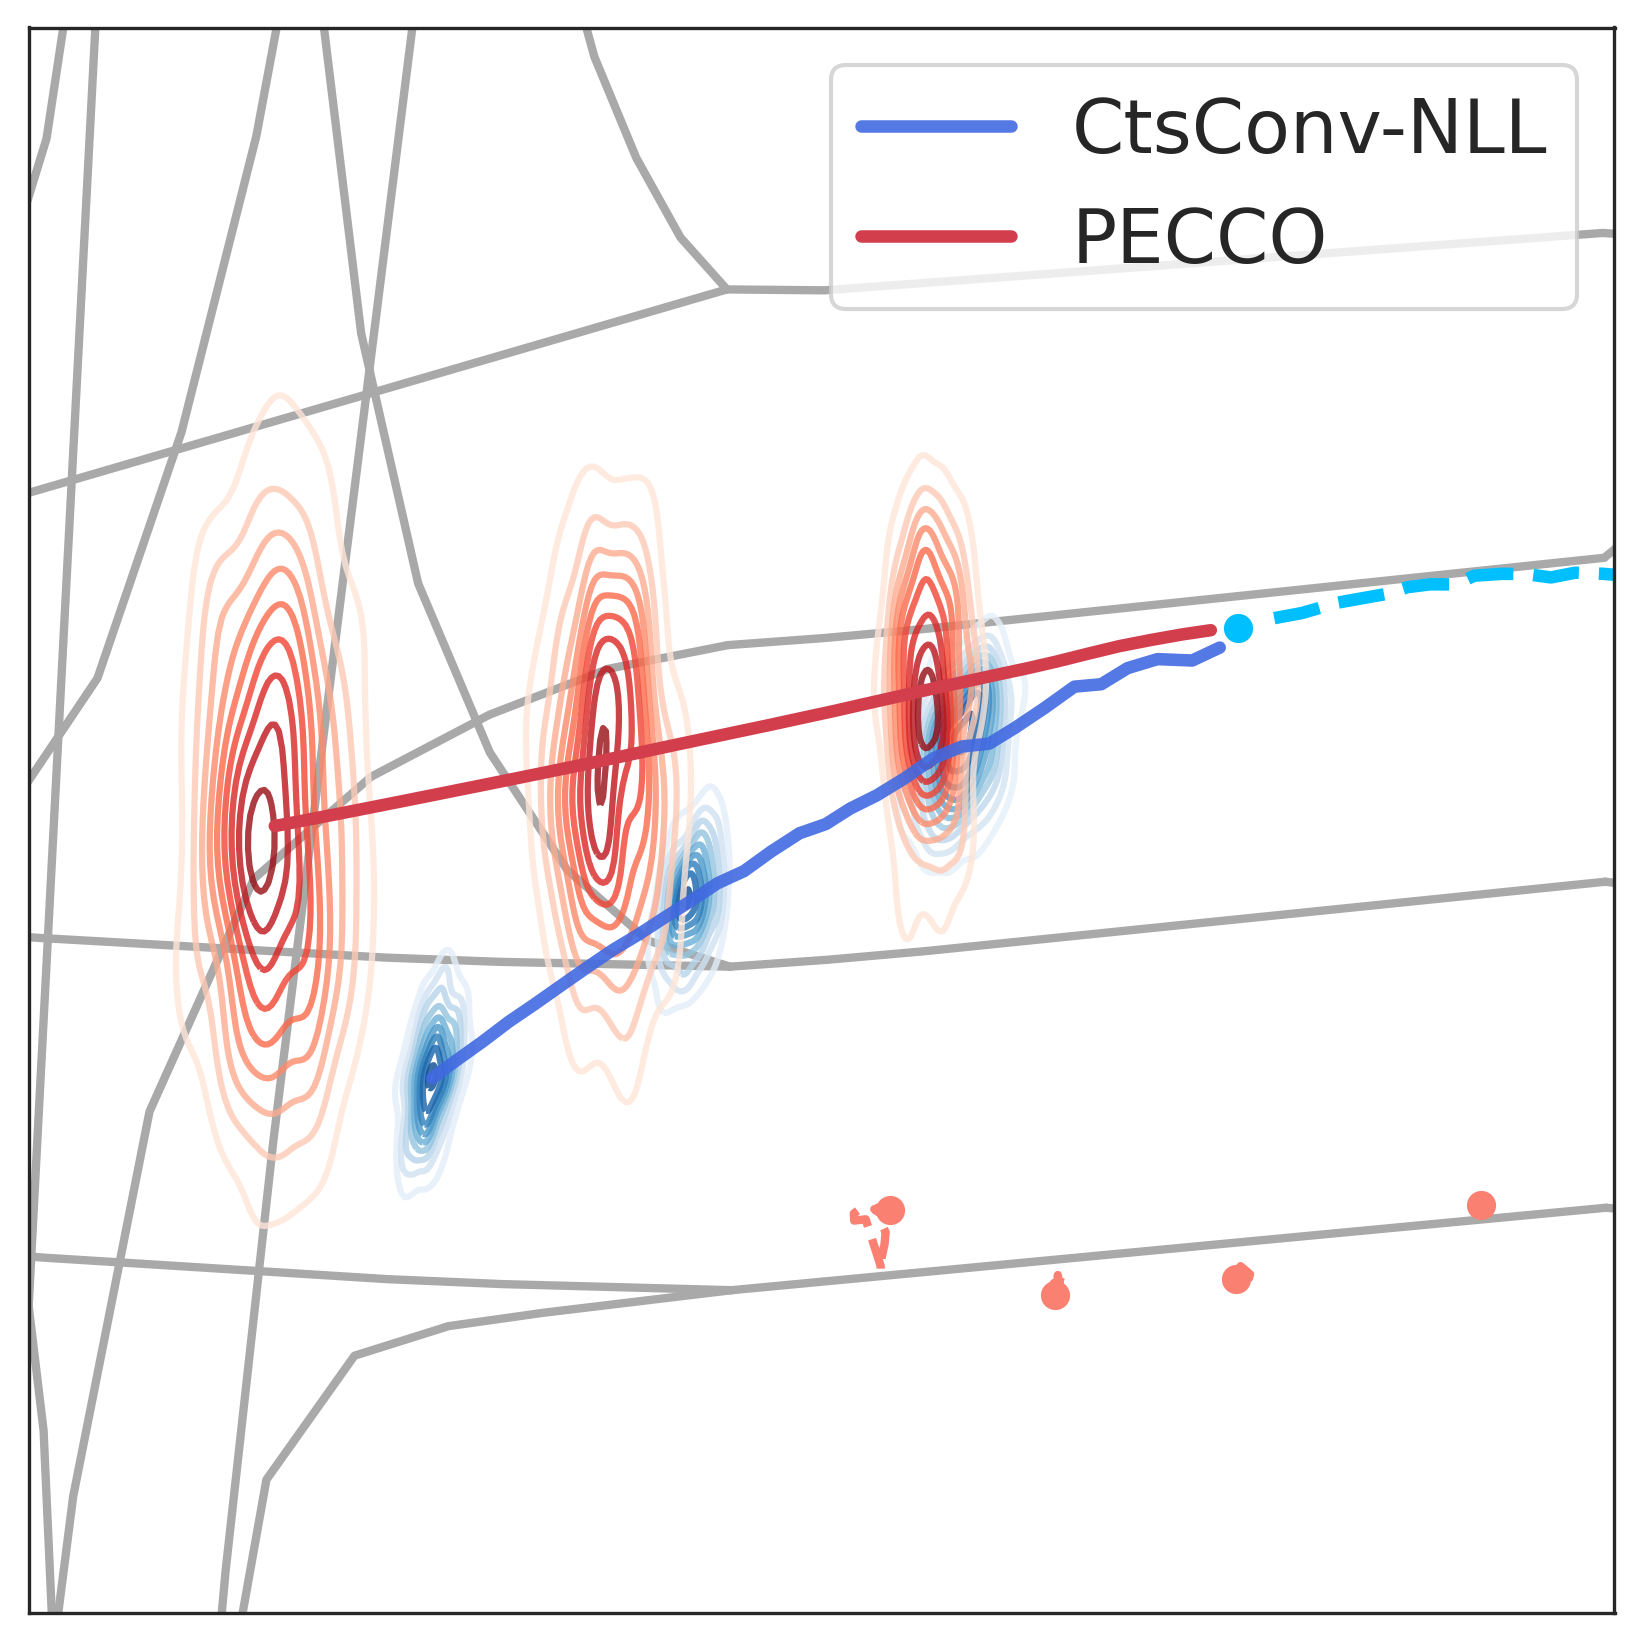
\includegraphics[width=\textwidth]{equivariance/figs/rot2.png}
        \caption{Rotated scene}
        \label{fig:eq0}
    \end{subfigure}
    \caption{Prediction on the same scene rotated by 90 degrees. PECCO is consistent in trajectory and uncertainty prediction, whereas the non-equivariant model (CtsConv) fails.}
    \label{fig:rotpred}
\end{figure}


In this paper, we propose a \textbf{P}robabilistic \textbf{E}quivariant \textbf{C}ontinuous \textbf{CO}nvolutional model (PECCO). PECCO is an equivariant probabilistic trajectory prediction model. Our key insight is to exploit \textit{symmetry} to estimate multidimensional conditional distributions with limited data.  We assume the predicted probability distribution is rotation and translation equivariant. That is, if the input data is transformed, the probability distribution will also be likewise transformed. In Figure \ref{fig:rotpred}, we see the same car approaching an intersection from either the south or east. The scenes are related by a $\pi/2$ rotation.  As the absolute compass direction is not particularly meaningful for local trajectory prediction, the model should thus output the same probability distributions over future trajectories for the car coming from the east as that coming from the north, but rotated by $\pi/2$.  Rotational equivariance not only allows our model to produce physically consistent predictions, the multiplicative nature of equivariance also allows us to model a probability space with a smaller sample size \cite{JMLR:v21:19-322}. For each sample which an equivariant model is trained on, an equivariant model learns as if it were trained on all transformations of that sample by the symmetry group \cite{wang2020incorporating}. 


PECCO also mitigates issues posed by other methods for enforcing equivariance such as data augmentation and normalization. Data augmentation adds rotated versions of data samples to the training dataset such that the model learns rotational equivariance. However, this slows training drastically, requires greater model capacity, and rarely achieves the level of equivariance or accuracy as equivariant neural networks \cite{trajectron++}. Data normalization is a technique that rotates the scene to the agent's reference frame for each data sample, as in \cite{vectornet}.  However, in the multi-agent setting, it is impossible to rotate the scene for multiple agents without a canonical reference frame. PECCO allows the weights to be relative to the local orientation of each agent without the need to rotate the scene repeatedly.   


Our main contributions are two folds: (1) We design an equivariant neural network, PECCO, for probabilistic forecast of multi-agent dynamics, and (2) we demonstrate that by incorporating symmetry, PECCO improves both calibration and sharpness of probabilistic forecasts on a synthetic particle dataset and two real-world benchmark datasets. 



% Effectively, we exploit a symmetry in the conditional probability distribution to factor out orientation, reducing dimensionality, and increasing the number of relevant samples for each prediction.  Intuitively, in order to make predictions for a given agent, our model will be able to generalize from similar samples in the training data regardless of which orientation or position those samples  occur in.     %that could be illustrated by showing say 10 samples in different orientations rotated to the same orientation to show a distribution.


  % Continuous convolution \cite{ummenhofer2019lagrangian} was designed \rw{has been used for} for particle-based fluid simulations. 
 %
%PECCO uses continuous convolution \cite{ctsconv} and enforces rotational equivariance as in \cite{ecco}, achieving more accurate and calibrated probabilistic forecasts. Continuous convolution generalizes discrete convolution and is useful for modeling interactions in many particle systems.

%   This way, our model is able to better estimate the probability for trajectory forecasts.
% Though similar  to graph convolution, like discrete convolution the weights are anisotropic and depend on the relative position of the two particles.   We use rotationally equivariant continuous convolutions as in \cite{ecco} in order to learn model weights which are relative to the local frame of each agent.  Our network is equivariant to rotation, translation, and permutation of particle labels, leading to improved coverage and consistency of predicted uncertainties. %generalization and consistency


% We evaluate our model on two datasets: Argoverse autonomous vehicle dataset \cite{argoverse} and TrajNet++ pedestrian trajectory forecasting challenge \cite{pedestriandata}. We demonstrate that in addition to enabling more accurate trajectory prediction, equivariance also improves the quality of uncertainty estimates in the context of trajectory prediction.


%\item We introduce a new metric, mean regional score (MRS), to evaluate the quality of probabilistic forecasts.
   

%In this work we present a multi-agent motion prediction model that are both equivariant and probablstic. 


% Trajectory prediction is one of the core tasks in AI,  from the movement of basketball players to fluid particles to car traffic \cite{sanchez2020learning, gao2020vectornet, shah2016applying}. 
% A common abstraction underlying these tasks is the movement of many interacting agents, analogous to  a many-particle system. Therefore,  understanding  the states of these particles, their  dynamics,  and hidden interactions is critical to accurate and robust trajectory forecasting.

% \begin{wrapfigure}{r}{0.5\textwidth}
% \vspace{-0.4cm}
%   \begin{center}
%     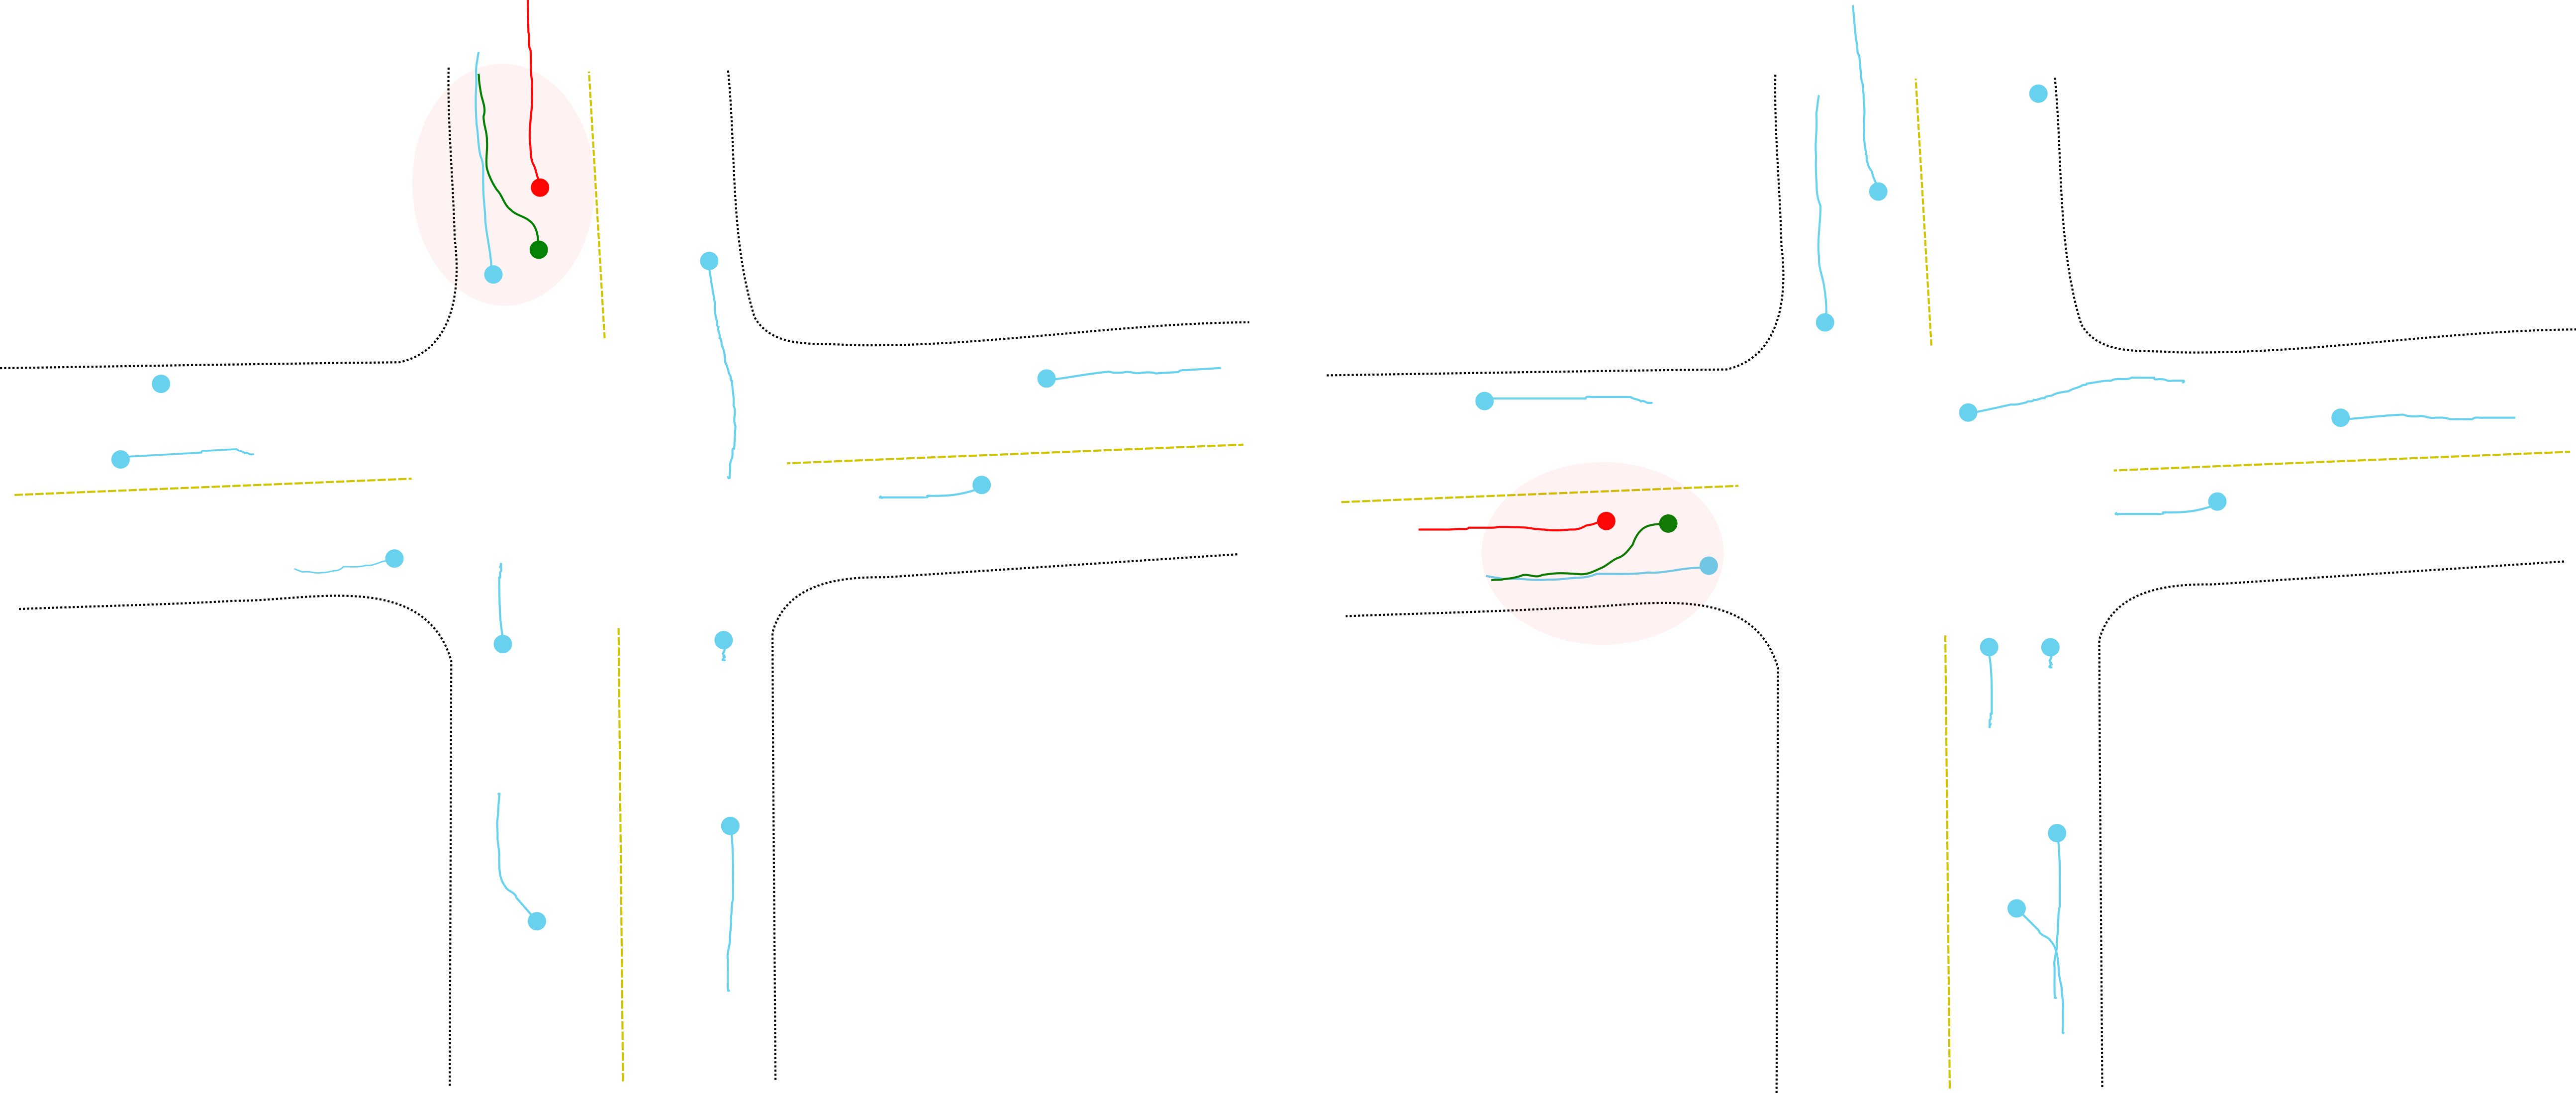
\includegraphics[width=0.5\textwidth,trim=40 30 40 20, clip]{figs/fig1.png}
%   \caption{Car trajectories in two scenes.  Though the entire scenes are not related by a rotation, the circled areas are.  \ours{} exploits this symmetry to improve generalization and sample efficiency.}
%   \end{center}
%   \vspace{-3mm}
%   \label{fig:twoscenes}
% \end{wrapfigure}

%  Even for purely physical systems such as in particle physics, the complex interactions among a large number of particles makes this a difficult problem.  For vehicle or pedestrian trajectories, this challenge is further compounded with latent factors such as human psychology.  Given these difficulties, current approaches require large amounts of training data and many model parameters. State-of-the-art methods in this domain such as %\cite{liang2020learning} and
%  \cite{gao2020vectornet}  
%  are based on graph neural networks. They do not exploit the physical properties of system and often make predictions which are not self-consistent or physically meaningful. Furthermore, they predict a single agent trajectory at a time instead of multiple agents simultaneously. %  \ry{need better argument}  
% % Furthermore, these methods adopt the perspective of a single agent in the scene, making it hard to produce consistent trajectories for all agents simultaneously. % 

% % \ry{this fig is taking too much space, make it compact}
% % \begin{figure}[b!]
% %     \centering
% %     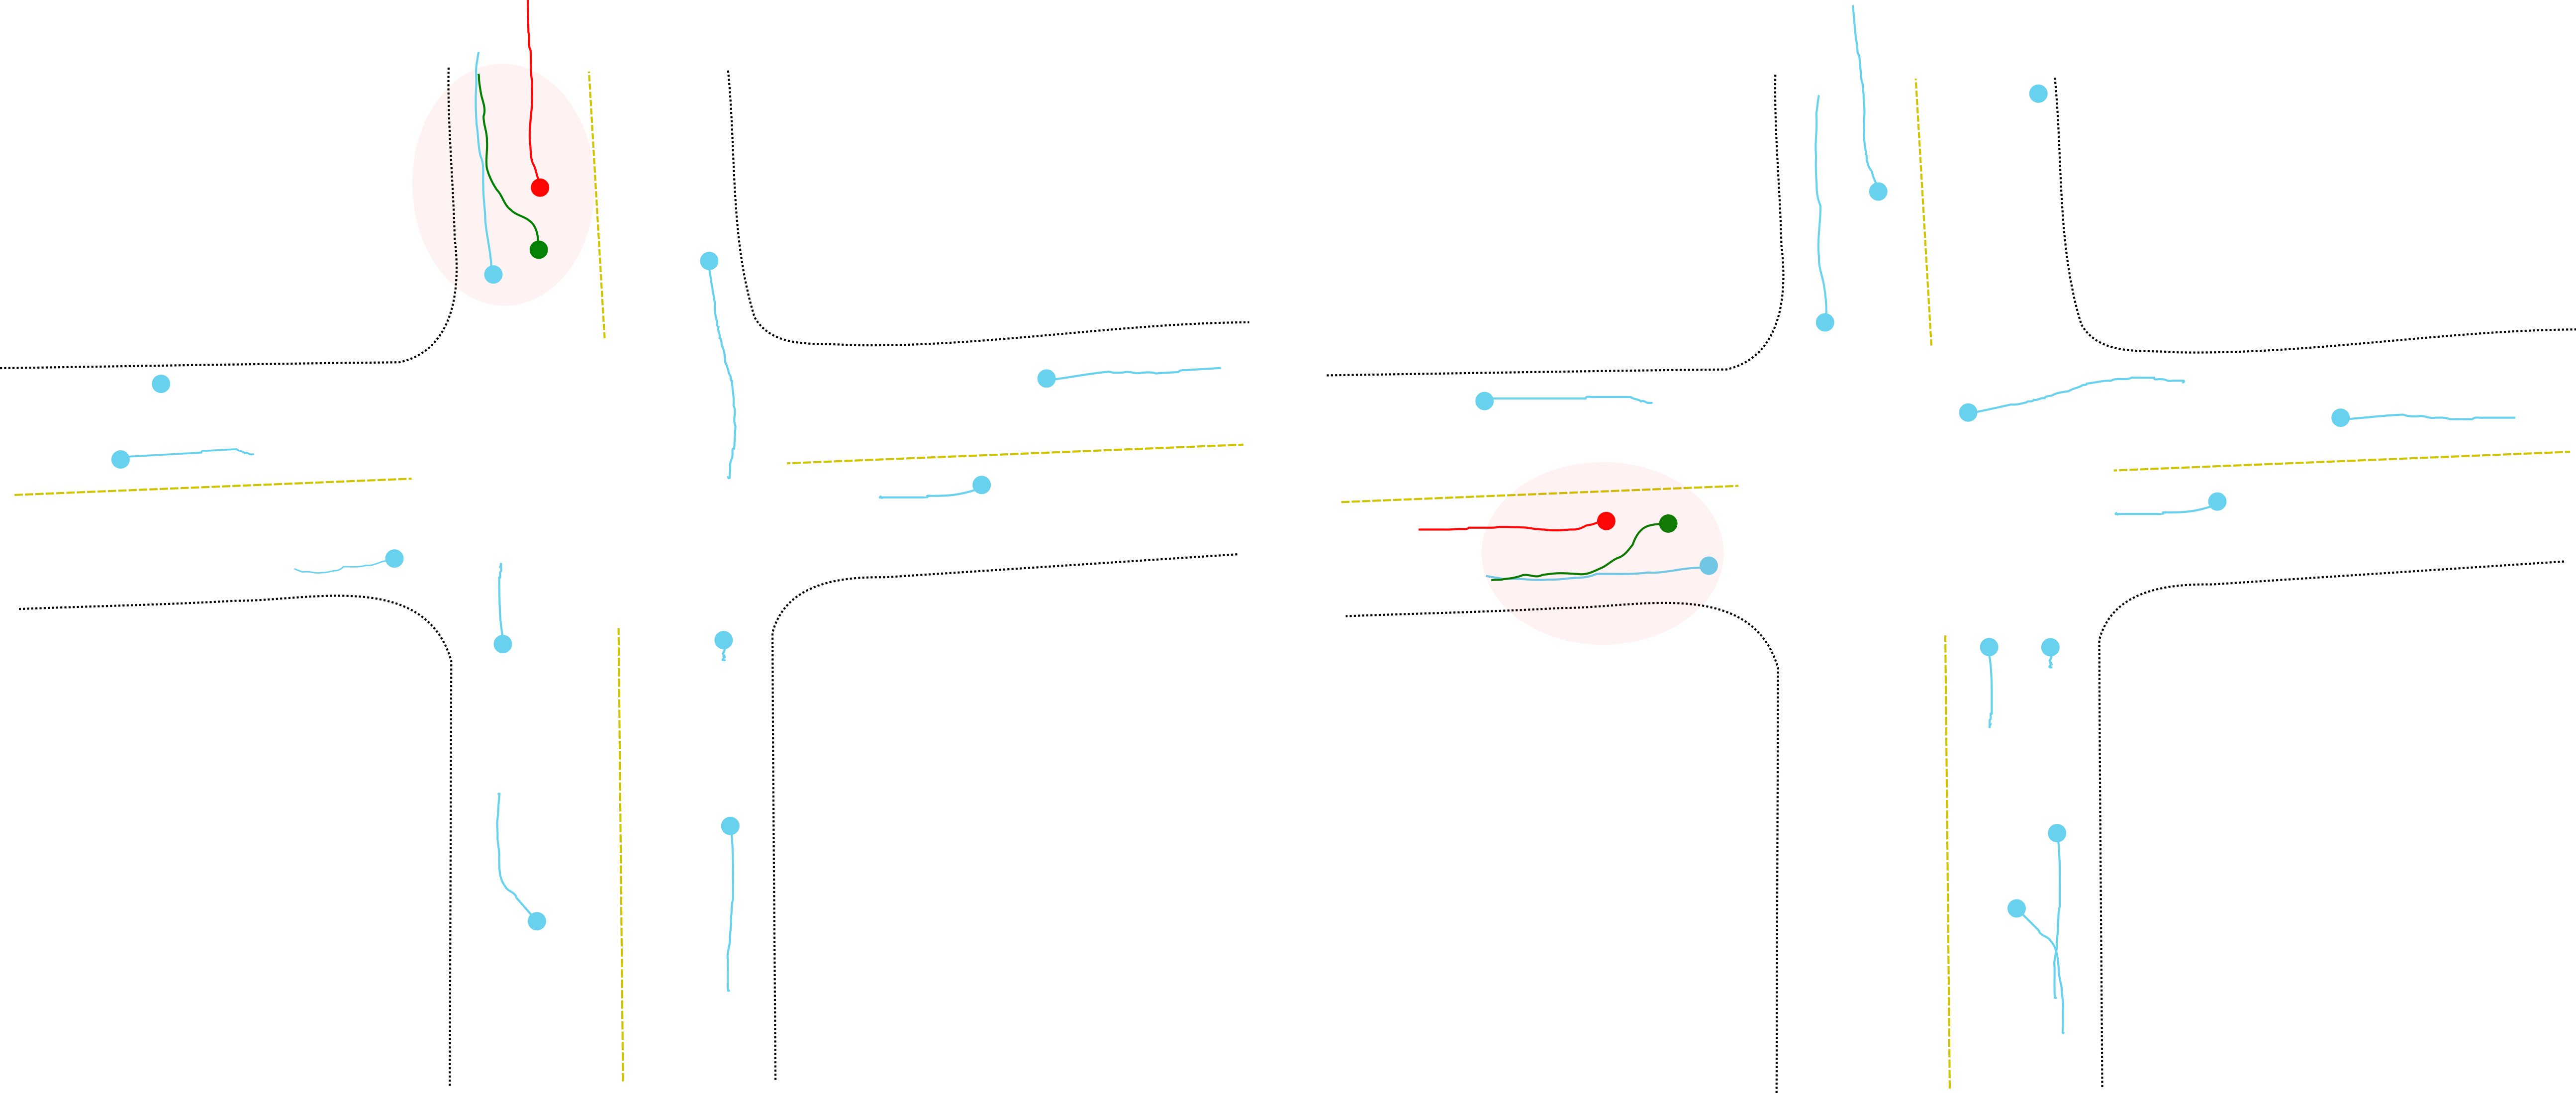
\includegraphics[width=10cm,trim=0 0 0 20, clip]{figs/fig1.png}
% %     \caption{Car trajectories in two scenes.  Though the entire scenes are not related by a rotation, the circled areas.  ECCO exploits this symmetry to improve generalization and sample efficiency.}
% %     \label{fig:twoscenes}
% % \end{figure}




% Our model is built upon a key insight of  many-particle systems pertaining to intricate internal symmetry. Consider a model which predicts the trajectory of cars on a road.  To be successful, such a model must understand the physical behavior of vehicles together with  human psychology. It should distinguish left from right turns, and give consistent outputs for intersections rotated with different orientation. As shown in \autoref{fig:twoscenes}, a driver’s velocity rotates with the entire scene, whereas vehicle interactions are invariant to such a rotation. Likewise, psychological factors such as reaction speed or attention may be considered vectors with prescribed transformation properties. Data augmentation is a common practice to deal with rotational invariance, but it cannot guarantee invariance and requires longer training. Since rotation is a continuous group, augmentation requires sampling from infinitely many possible angles.

% %  In our model, this is achieved by considering all hidden layers to be vectors with the prescribed action of a symmetry group.



% In this paper, we propose an equivariant continuous convolutional model, \ours{}, for trajectory forecasting. % Continuous convolution \cite{ummenhofer2019lagrangian} was designed \rw{has been used for} for particle-based fluid simulations. 
%  %
%  Continuous convolution generalizes discrete convolution and is adapted to data in  many-particle systems with complex local interactions. \citet{ummenhofer2019lagrangian} designed a model using continuous convolutions for particle-based fluid simulations.
% %
% Meanwhile, equivariance to group symmetries has proven to be a powerful tool to integrate physical intuition  in physical science applications  \cite{wang2020incorporating, brown2019equivariant, kanwar2020equivariant}.  Here, we test the hypothesis that an equivariant model can also capture internal symmetry in non-physical human behavior. Our model utilizes a novel weight sharing scheme, torus kernels, and is rotationally equivariant.

% %  We perform an ablative study to validate the importance of different aspects of our model.
  
% We evaluate our model on two real-world trajectory datasets: Argoverse autonomous vehicle dataset \cite{chang2019argoverse}  and TrajNet++ pedestrian trajectory forecasting challenge \cite{kothari2020human}.       We demonstrate on par or better prediction accuracy to baseline models and data augmentation with fewer parameters, better sample efficiency, and stronger generalization properties.  Lastly, we demonstrate theoretically and experimentally that our polar coordinate-indexed filters have lower equivariance discretization error due to being better adapted to the symmetry group.  

% Our main contributions are as follows:
% \begin{itemize}
%     \item We propose \textbf{E}quivariant \textbf{C}ontinous \textbf{CO}nvolution (\ours{}), a rotationally equivariant deep neural network that can capture internal symmetry in trajectories. 
%     \item We  design \ours{} using a novel weight sharing scheme based on orbit decomposition and polar coordinate-indexed filters. We implement equivariance for both the standard and regular representation $L^2(\mathrm{SO}(2))$.
%     \item On benchmark Argoverse and TrajNet++ datasets, \ours{} demonstrates  comparable accuracy  while enjoying better generalization, fewer parameters, and better sample complexity.
%     % \item We demonstrate theoretically and experimentally that despite discretization our polar coordinate-indexed filters have very low equivariance error. \ry{not clear the significance}  
% \end{itemize}
